\chapter{\textit{Background}}
Este trabalho aborda, principalmente, três conceitos. O primeiro diz respeito ao tipo de site que foi investigado e ao qual se tentou propor alguma melhoria de design. O segundo se refere ao ato de coletar algum tipo de informação utilizando, como auxílio, as conexões sociais estabelecidas entre indivíduos, como, por exemplo, fazer uma pergunta a amigos no \textit{Facebook}. Tal recurso está ligado com a possível melhoria de design estudada durante este trabalho. O terceiro conceito envolve um tipo de custo relacionado ao uso deste recurso. Portanto, faz-se necessário apresentar neste capítulo: um levantamento em mais detalhes dos significados destes três conceitos, bem como uma visão geral do que já estava abordado na literatura em relação aos mesmos e que é, de certa forma, relevante para esta pesquisa.

\section{Sites \qa}
Definiu-se para o escopo detste trabalho o conceito de sites \qanospace, que são aqueles os quais são acessados por usuários com o intuito de: realizar perguntas, responder a perguntas, realizar comentários sobre perguntas, respostas e até mesmo outros comentários ou, ainda, visualizar as discussões geradas por perguntas e os seus respectivos conjuntos de respostas (ver a Figura~\ref{fig:casosdeusositesqa}). Os sites \qa são classificados na literatura de duas maneiras distintas: \textit{community} \qa e \textit{social} \qa \cite{gazan2011social}.

\textit{Community} \qa é um termo de uso específico: para um site ser classificado assim, é preciso que haja uma identificação de indicadores formais de comunidade, como usuários se mostrando engajados em divulgá-lo, adotando e expressando uma identidade, etc. \cite{kling2005understanding} Tal classificação é, muitas vezes, feita de forma indiscriminada \cite{rosenbaum2010structuration}.

    \begin{figure}[H]
        \center
        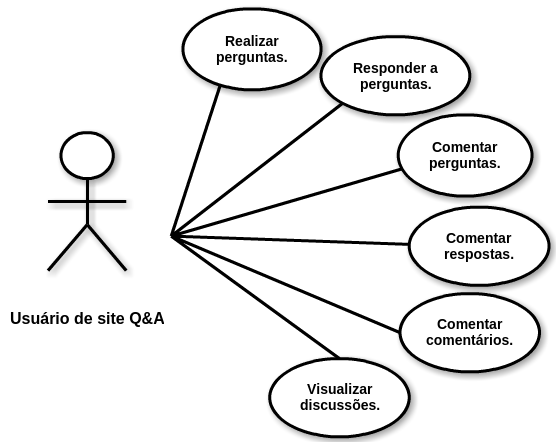
\includegraphics[scale=.5]{./figuras/casosdeusositesqa.png}
        \caption{Casos básicos de uso de um site \qanospace.}
        \label{fig:casosdeusositesqa}
    \end{figure}


\textit{Social} \qanospace, de acordo com Gazan et al. \cite{gazan2011social}, aparece como um termo mais abragente e se refere aos sites nos quais os respectivos usuários realizam perguntas, respondem a perguntas e avaliam o conteúdo do site enquanto estão interagindo com ele. Apesar de sites deste tipo serem considerados instâncias de comunidades \textit{online} \cite{rosenbaum2010structuration}, o que pode remeter ao conceito de \textit{community} \qanospace, a maior parte dos trabalhos utilizados na elaboração da fundamentação teórica desta pesquisa e, portanto, relevantes neste escopo, opta por utilizar o conceito de \textit{social} \qanospace. Tal opção também foi escolhida durante a elaboração desta dissertação. Portanto, no âmbito desta pesquisa, sites \qa  são, também, definidos como sites do tipo social \qanospace.

Utilizando o \textit{Stack Overflow em Português} (a Figura~\ref{fig:perguntasopt} auxilia nesta ilustração), é possível descrever o modelo de funcionamento de um site \qa, tal qual foi descrito na literatura por Furtado et al. \cite{furtado2013contributor}:
    \begin{itemize}
        \item Um dado usuário publica alguma pergunta descrevendo um problema;
        \item A pergunta criada é listada no site e visualizada por outros usuários, que podem votar sobre a utilidade ou não da questão, assim como marcá-la como um tópico favorito;
        \item Qualquer usuário pode publicar respostas e comentários que ficam relacionados com a pergunta;
        \item Os demais usuários do site podem visualizar as respostas e comentários, que também podem receber votos;
        \item Comentários neste contexto são utilizados como ferramenta para discussão e esclarecimento entre o usuário que publicou a pergunta (perguntador) e os demais membros do site;
        \item Finalmente, o perguntador pode selecionar uma das respostas como sendo a melhor.
    \end{itemize}
    
Os 3 campos primários de pesquisa em sites \qa presentes na literatura até então são: estudos sobre motivações e comportamentos dos usuários, avaliações da qualidade da informação contida nestes sites e análises de fatores tecnológicos que exercem influência na participação de usuários \cite{shah2009research}.

Este trabalho está relacionado com o campo de avaliações da qualidade da informação, pois houve um esforço para se realizar uma análise quantitativa sobre o efeito do compartilhamento em redes sociais na obtenção ou não de respostas úteis para os autores das perguntas compartilhadas.

Existem trabalhos que investigam maneiras de melhorar a qualidade das respostas contidas em sites \qa fomentando-os de alguma forma \cite{harper2008predictors,chen2010knowledge,jeon2010re}. Todas estas pesquisas envolvem estudar como o oferecimento de algum tipo de recompensa, inclusive monetária, pode atrair respostas ou melhorar a qualidade das mesmas. Há um consenso de que, oferencendo algum tipo de recompensa ou vantagem para os usuários, é possível aumentar significativamente o número de respostas obtidas para as perguntas realizadas em sites \qanospace. Entretanto, um aumento grande e repentino de contribuições em sites \qa geralmente não serve para melhorar a qualidade das respostas.

No âmbito da avaliação da qualidade do conteúdo em sites \qanospace, aparecem alguns trabalhos interessantes e bastante citados porque analisam o que faz perguntas e respostas atraírem o interesse de outros usuários. R. Gazan \cite{gazan2006specialists} concluiu que as respostas mais gerais e resumidas tendem a receber mais votos positivos do que aquelas mais específicas e detalhadas que são dadas por especialistas, dando a entender que há uma preferência por informações que são assimiladas com mais rapidez e facilidade.

Segundo  Harper et al. \cite{harper2009facts} os usuários de sites \qa conseguem distinguir questões de conversão de questões factuais. Uma típica questão de conversação é aquela cujo intuito é iniciar algum debate e não é possível estabelecer, de forma precisa, se uma dada resposta está certa ou errada. As factuais, por sua vez, são aquelas cujas respostas podem ser classificadas como certas ou erradas. A Figura~\ref{fig:conversa} e a Figura~\ref{fig:factual} contêm exemplos de perguntas destes tipos no site \textit{Quora}. De acordo com este trabalho, há evidências de que se uma questão for factual, então ela possui mais chances de permanecer guardada nos arquivos de um site \qanospace, além de possivelmente agradar a um maior número de usuários deste tipo de site.

    \begin{figure}[H]
        \center
        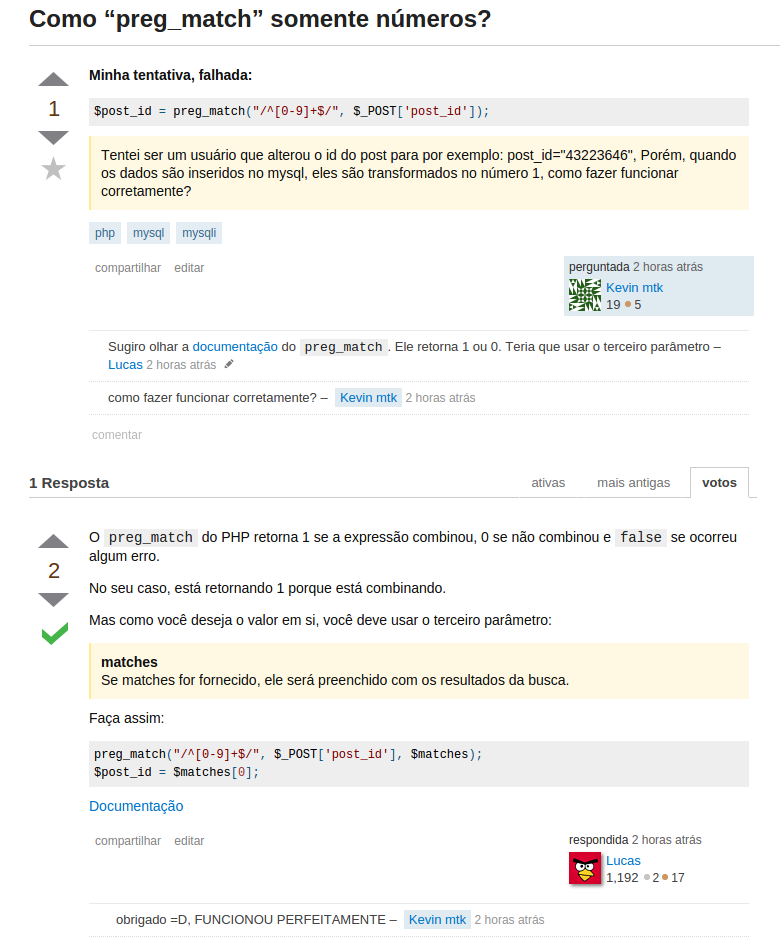
\includegraphics[scale=.5]{./figuras/exemplo-so-pt.png}
        \caption{Página referente a uma questão no \textit{Stack Overflow em Português}.}
        \label{fig:perguntasopt}
    \end{figure}


    \begin{figure}[H]
        \center
        
\includegraphics[scale=.8]{./figuras/conversa.png}
        \caption{Exemplo de uma pergunta de conversação no \textit{Quora}.}
        \label{fig:conversa}
    \end{figure}
    
    \begin{figure}[H]
        \center
        
\includegraphics[scale=.8]{./figuras/factual.png}
        \caption{Exemplo de uma pergunta factual \textit{Quora}.}
        \label{fig:factual}
    \end{figure}


% Existem ainda alguns trabalhos importantes e relevantes que discorrem sobre métricas utilizadas para se determinar a qualidade das respostas obtidas em sites \qa \cite{gazan2011social}. De acordo com a literatura, não houve nenhum esforço, até aqui, para saber a influência do ato de compartilhar perguntas de sites \qa em redes sociais na qualidade das respostas obtidas.

% É evidente, portanto, que existia na literatura, até a realização desta pesquisa de mestrado, uma oportunidade em aberto de tentar relacionar o compartilhamento em redes sociais com a qualidade e quantidade do conteúdo gerado em sites \qanospace.

% Fica claro que havia, até a realização deste mestrado, uma lacuna na literatura sobre a questão de se compartilhar em redes sociais perguntas oriundas de sites \qanospace. Houve, nesta pesquisa, um esforço para tentar descobrir se compartilhar perguntas de sites \qa nas redes sociais pode ajudar ou não a fomentar tais sites com respostas satisfatórias para os donos das perguntas compartilhadas.

A pesquisa de mestrado presente também está inserida no campo dos estudos sobre motivações e comportamento dos usuários, tendo em vista que abordou a maneira com a qual usuários de sites \qa lidam com a funcionalidade de compartilhar perguntas em redes sociais contida em tais ambientes.

Já foi mostrado anteriormente na literatura evidências de que as estruturas de recompensas sociais presentes em sites \qanospace, como a obtenção de pontos e reputação de acordo com o número de perguntas ou respostas publicadas, formam um ponto crítico para o sucesso e bom funcionamento destes ambientes \cite{shah2008exploring}. 

Huang et al. discorreram, em um trabalho anterior \cite{li2012quantifying}, sobre o efeito destas recompensas sociais na participação dos usuários em tais sites. Utilizando dados do \textit{Stack Overflow}, eles encontraram correlação entre o número de recompensas sociais (conhecidas como medalhas ou \textit{badges}) e o aumento da motivação que os usuários têm para contribuir com o site. 

De acordo com uma análise realizada durante o trabalho supracitado, as frequências de todos os tipos de atividades possíveis dentro do site estudado estão correlacionadas com as quantidades das respectivas recompensas sociais oferecidas pelo site. Eles concluíram que quanto maior for o número de \textit{badges} relacionadas com uma dada atividade dentro do \textit{Stack Overflow}, mais motivados os usuários se sentirão para realizá-la. Portanto, o baixo número de \textit{badges} que os usuários podem ganhar ao compartilhar perguntas do \textit{Stack Overflow em Português} nas suas redes sociais talvez explique, em partes, o motivo pelo qual tal prática não é recorrente. Esta pesquisa de mestrado encontrou outros fatores que auxiliam a explicação de tal fato.

É interessante constatar que existe, não só no site \textit{Stack Overflow em Português}, mas também em vários outros, uma forma de recompensar usuários que compartilham perguntas destes sites em redes sociais (ver Figura~\ref{fig:medalhassopt}).

    \begin{figure}[H]
        \center
        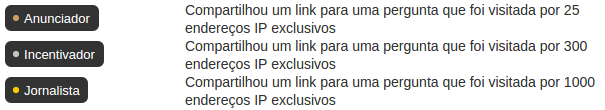
\includegraphics[scale=.5]{./figuras/medalhas-compartilhar-sopt.png}
        \caption{As \textit{badges} oferecidas pelo \textit{Stack Overflow em Português} aos usuários que compartilham perguntas deste site em redes sociais.}
        \label{fig:medalhassopt}
    \end{figure}

Alguns trabalhos também analisam padrões de participação e de comportamento dos usuários \cite{adamic2008knowledge,furtado2013contributor,bian2008few}. Estudou-se os tipos mais comuns de usuários e o que eles faziam de especial: os que apenas perguntavam, os que apenas respondiam, aqueles que só colaboravam de forma específica em certos tipos de postagens, etc. Nenhuma informação foi encontrada, nestes trabalhos, a respeito dos usuários que compartilham perguntas destes sites nas redes sociais.

É natural, então, constatar a lacuna que havia na literatura acerca de trabalhos que relacionam o compartilhamento em redes sociais de perguntas de sites \qa com: motivações e comportamento dos usuários, tipos de perguntas realizadas em sites \qa e redes socias e, também, com a qualidade e quantitade de respostas obtidas para perguntas realizadas em tais sites. Esta pesquisa de mestrado oferece contribuições pontuais para áreas da literatura discorridas nesta seção, ao passo que houve um esforço para encontrar respostas para os seguintes questionamentos:

    \begin{itemize}
        \item Compartilhar perguntas de sites \qa em redes sociais pode, de fato, ajudar a atrair mais respostas para tais perguntas?
        \item Compartilhar perguntas de sites \qa em redes sociais, pode, de fato, ajudar a melhorar a qualidade das respostas obtidas para tais perguntas?
        \item O que pode fazer uma pergunta oriunda de um site \qa ser ou não compartilhada em redes sociais por um dado usuário que não é, necessariamente, o autor original da pergunta? 
        \item Como os usuários de sites \qa enxergam a atividade de compartilhar, em redes sociais, perguntas oriundas de tais sites? Eles acreditam que isto funciona? Por quê? Eles constumam fazer isto? Por quê?
    \end{itemize}

\section{\textit{Friendsourcing}}
\textit{Crowdsourcing} é um conceito que representa o processo no qual soluções criativas são extraídas de um grupo de indivíduos que se disponibilizam para oferecer algum serviço a partir de uma convocação realizada por parte de quem precisa de tal serviço \cite{brabham2008crowdsourcing}. Por exemplo, imagine um empresa que faça vendas \textit{online} de camisetas cujas estampas são escolhidas por meio de uma competição entre \textit{designers} do mundo todo que estejam querendo mostrar seus trabalhos. Este exemplo existe na prática: é a empresa \textit{Threadless}\footnote{https://www.threadless.com/}.

Usualmente, \textit{crowdsourcing} está relacionado com o recrutamento \textit{online} de indivíduos dispostos a realizar uma tarefa que seria muito trabalhosa ou difícil se fosse feita por uma única pessoa. Em sites que utilizam este conceito, um grande número de usuários incrementam os conteúdos globais destes sites por meio de pequenas contribuições pontuais \cite{Bernstein:2008:PVF:1746259.1746260}. Portanto, é possível afirmar que sites \qa utilizam \textit{crowdsourcing} como forma de fornecer o serviço prometido: encontrar uma resposta para uma dada pergunta realizada por algum usuário.

A partir do supracitado, aparece o conceito de \textit{friendsourcing}: uma forma de \textit{crowdsourcing} na qual se visa coletar informação disponível em grupos pequenos e socialmente conectados de maneira precisa \cite{Bernstein:2008:PVF:1746259.1746260}. Tais grupos podem ser, por exemplo, formados por amigos de quem está solicitando o serviço. Um exemplo de \textit{friendsourcing} é alguém perguntar algo aos seus amigos no \textit{Facebook} por meio de uma publicação que esteja visível a todos eles. 

% Existiam, até aqui, trabalhos cujos esforços se basearam em relacionar \textit{friendsourcing} com a realização de perguntas em redes sociais de uma forma diferente do que está nesta dissertação de mestrado. 
Alguns pesquisadores propuseram melhorias na busca em redes sociais por amigos que são capazes de oferecer algum serviço solicitado, como Savage et al. \cite{Savage:2012:DSQ:2380296.2380321}. Neste trabalho se criou uma ferramenta capaz de auxiliar usuários que desejam requisitar de amigos em redes sociais algum tipo de auxílio, mas que esbarram no problema de se ter uma lista grande de amigos e não saber quem são aqueles com capacidade e interesse em ajudar, o que dificulta a busca por pessoas nesta lista para que esta requisição seja feita de forma direta. A ferramenta desenvolvida se mostrou útil do ponto de vista dos usuários. Eles relataram que ficaram satisfeitos com a listagem de todos os amigos que poderiam, de certa forma, ter a ver com os temas das perguntas realizadas. 

Na pesquisa realizada por Brady et al. \cite{Brady:2013:IAS:2441776.2441915} se investigou como as pessoas cegas utilizam as redes sociais para tirar dúvidas cotidianas como, por exemplo, perguntar aos amigos quais são as cores das flores presentes em um vaso mostrando uma foto dele. Descobriu-se que, de fato, as redes sociais são muito utilizadas por usuários cegos com tal finalidade. Entretanto, ficou constatato que tais usuários não acham que as redes sociais são os lugares mais apropiados para tal atividade, pois eles demonstraram ter bastante receio em incomodar os amigos e, além disto, não há garantias de que seus amigos irão ajudá-los em tempo hábil.

Existem, na literatura, trabalhos nos quais os pesquisadores buscam compreender como se dá o processo de perguntar a amigos em redes sociais. Paul et al. \cite{paul2011question}, por exemplo, conduziram uma pesquisa com o intuito de se categorizar as perguntas realizadas no \textit{Twitter}. De acordo com os resultados obtidos, os tipos mais populares de perguntas encontrados foram: perguntas retóricas, perguntas factuais e enquetes. Ainda de acordo com tal pesquisa, entretenimento, saúde e tecnologia foram os temas mais recorrentes.  

Seguindo a ideia da pesquisa supracitada, Morris et al. \cite{morris2010people} realizaram um estudo mais amplo com o intuito de observar o comportamento dos usuários das duas redes sociais mais populares da Internet (\textit{Facebook} e \textit{Twitter}) em relação ao ato de realizar perguntas nestes ambientes. Foram elencados os tipos mais comuns de perguntas realizadas, bem como as motivações dos usuários que perguntam nestas redes sociais, por meio de um questionário respondido por mais de 600 usuários que trabalhavam na empresa \textit{Microsoft}\footnote{http://www.microsoft.com/}. Confiança nos amigos e os aspectos subjetivos das perguntas realizadas (é mais fácil pedir opinião pessoal para amigos) foram as duas principais motivações para os usuários realizarem perguntas nas redes sociais. Os temas sobre tecnologia, entretenimento e questões domésticas e familiares foram as mais recorrentes. Os tipos de perguntas mais presentes foram as perguntas subjetivas (pedido de recomendação ou opinião) e as factuais.

É importante ressaltar que todos os trabalhos existentes até então que relacionaram \textit{friendsourcing} e o ato de perguntar na Internet são do ponto de vista de quem faz a pergunta. Não havia, até aqui, nenhum trabalho que abordasse a perspectiva de quem utiliza \textit{friendsourcing} nas redes sociais sem, necessariamente, estar querendo beneficiar a si mesmo. Nesta pesquisa de mestrado houve um esforço para investigar as motivações dos usuários que utilizaram \textit{friendsourcing} em perguntas oriundas de sites \qa cujos autores nem sempre eram eles mesmos. Além disto, também procurou-se averiguar quais eram os tipos das perguntas compartilhadas.

Fica constatada, portanto, esta sutil lacuna na literatura que também se abordou durante esta pesquisa de mestrado quando se investigou o uso de \textit{friendsourcing} (compartilhamento de perguntas em redes sociais) como tentativa de fomentar sites \qanospace.

\section{Capital Social}
Capital social, apesar de apresentar várias definições na literatura, pode ser entendido como um tipo de benefício decorrente da participação em redes ou outras estruturas sociais, sendo utilizado para facilitar novas interações sociais \cite{portes2000social}.

Sendo assim, de acordo com a definição acima, entende-se que, dentro de uma dada rede social, toda e qualquer interação entre indivíduos representará ganho e/ou perda de capital social para alguém. Por exemplo, quando um dado usuário pergunta algo para os seus seguidores no \textit{Twitter} (usuários que acompanham as suas publicações nesta rede), espera-se que aquele que fornecer uma resposta útil ganhará capital social em relação ao usuário autor da pergunta. Por outro lado, também espera-se o seguinte: um certo usuário perde cada vez mais capital social à medida que solicita ajuda a outros em uma dada rede social sem nunca oferecer nada em troca. 

Portanto, é coerente relacionar o conceito de \textit{friendsourcing} com o de capital social, como foi feito por Rzeszotarski et al. \cite{rzeszotarski2014estimating} em um trabalho no qual se tentou investigar como os usuários de redes sociais enxergam os custos sociais envolvidos na realização de perguntas em redes sociais. Ficou constatado que os usuários enxergam altos custos sociais com relação ao uso das redes sociais para se realizar perguntas. Embora tenha-se verificado que os usuários não se mostraram tão preocupados assim em incomodar os amigos, como foi observado em outros trabalhos, foi possível constatar que em vários momentos os participantes relataram que preferiam pagar em dinheiro do que gastar capital social para encontrar alguma resposta.   

Vários trabalhos na literatura tentaram investigar o uso de capital social em redes sociais na Internet. Valenzuela et al. \cite{valenzuela2009there} tentaram descobrir se o uso do \textit{Facebook} estava relacionado com o ganho de capital social no cotidiano dos seus usuários por meio de medições de variáveis relacionadas, segundo a sociologia, com capital social, como: participação política, satisfação de vida, engajamento civil, etc. Observou-se que existe uma correlação positiva entre tais fatores.

Burke et al. \cite{Burke:2011:SCF:1978942.1979023} estudaram como os diferentes tipos de uso de uma rede social grande e popular como o \textit{Facebook} estão relacionados com o conceito de capital social. Neste estudo foi examinado como as seguintes ações estão relacionadas com ganhos e perdas de capital social: comunicação direta entre amigos, \textit{broadcast} de mensagens e leitura de conteúdos publicados por terceiros. Apenas a comunicação direta entre amigos se mostrou estar relacionada com o ganho de capital social entre usuários. \textit{Broadcast} de mensagens e leitura de conteúdos publicados por terceiros não afetaram, diretamente, as relações entre os usuários. Ou seja: não houver ganhos ou perdas significativos de capital social nestes casos.

Recuero et al. \cite{recuero2012economia} tentaram relacionar o acesso à informação no \textit{Twitter} com o conceito de capital social. Os resultados deste trabalho sugerem que algumas práticas geram benefícios individuais e coletivos nos quais as replicações de mensagens, ou os \textit{retweets}, atuam como moeda de troca. Há um consenso de que, no \textit{Twitter}, um dos maiores objetivos dos usuários é ter suas mensagens visualizadas pela maior quantidade possível de pessoas dentro da rede. Os pesquisadores discutem que replicar as mensagens de amigos gera ganho de capital social que, posteriormente, pode ser utilizado para replicar novas mensagens, resultando em uma espécie de círculo vicioso.

Atentando para a lacuna existente na literatura, é importante ressaltar que, nesta pesquisa de mestrado, houve um esforço para se estudar como o conceito de capital social está relacionado com o compartilhamento em redes sociais de perguntas oriundas de sites \qanospace. Não foi identificado nehum estudo neste sentido até então. Durante as investigações qualitativas desta pesquisa, procurou-se entender como os usuários enxergavam o capital social relacionado com o compartilhamento de perguntas originalmente publicadas em outros sites e cujos autores muitas vezes não eram eles mesmos.